\chapter{Occupancy\label{sec:occ_proj}}


\begin{center}
\textbf{Submit via MMS before midnight on Monday the 13th April }\footnote{The School lateness penalty policy is as follows: A late piece of work is penalised with an initial penalty of 15\% of the maximum available mark (or 3 marks if anyone is marking on the University's 20-point scale), and then a further 5\% (1 mark on the 20-point scale) per 8-hour period, of part thereof.}
\end{center}

\subsection*{The Datasets}

The file \verb|swtdat.rda| in folder ``\verb|Exercises and Projects|'' on MMS contains presence/absence data on Swiss willow tits from the Swiss Survey of Common Breeding Birds. This is an annual survey conducted during the breeding season. Sample units are 1km$^2$, and these are sampled 2 or 3 times by each volunteer observer. The observers survey on foot a route of variable length between quadrats, but the same length on different occasions within each quadrat. Observers choose the intensity of sampling themselves, i.e., the duration of their survey along the route. Surveys of each quadrat typically happened on different days and the data include the day on which each quadrat was surveyed on each occasion.

Two covariates believed to be of biological relevance are elevation and forest cover. These are thought to be important determinants of distribution and abundance. Elevation gradient is severe in Switzerland and this substantially affects climate, weather and vegetation. Elevation and forest cover are illustrated in Figures~\ref{fig:elevation} and \ref{fig:forest}.

\begin{figure}
\caption{Elevation of Switzerland in metres above sea level.\label{fig:elevation}}
\centering
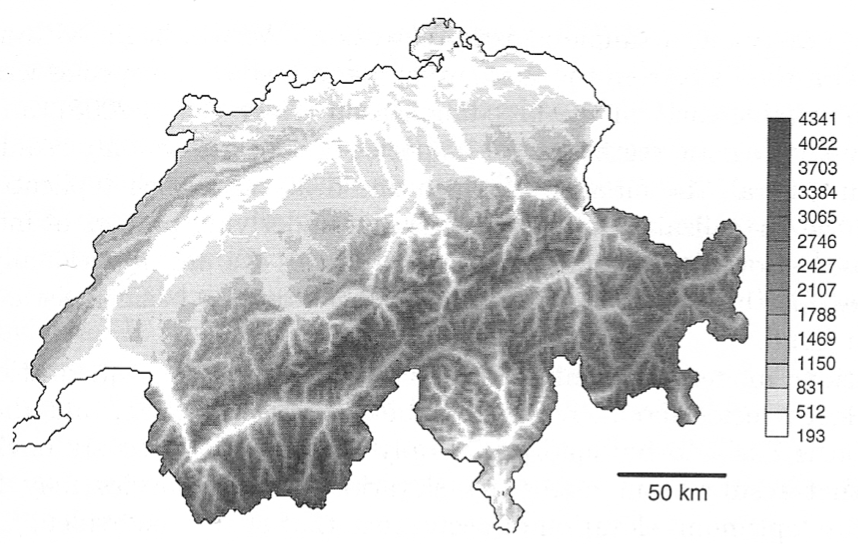
\epsfig{file=elevation.png,width=12cm}
\end{figure}

\begin{figure}
\caption{Forest cover of Switzerland  (percent of quadrat that is forested).\label{fig:forest}}
\centering
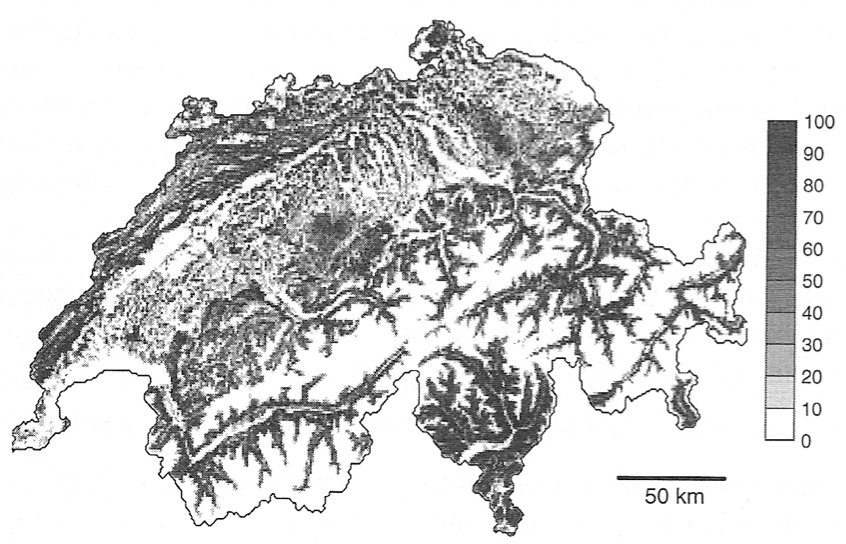
\epsfig{file=forest.png,width=12cm}
\end{figure}

The variables in \verb|swtdat.rda| are as follows:

\begin{description}
\item[ch] Capture history in \verb|Rmark| format (``.'' means no survey of that quadrat on the occasion).
\item[elev] Elevation difference from mean elevation (1182.574 m), in metres.
\item[elevsq] Square of elev.
\item[forest] Percentage of quadrat covered in forest.
\item[dur1] Duration of search on occasion 1, in minutes.
\item[dur2] Duration of search on occasion 2, in minutes.
\item[dur3] Duration of search on occasion 3, in minutes.
\item[length] Length of route searched, in km.
\item[intensity1] Intensity of search (duration/length) on occasion 1, in minutes per km.
\item[intensity2] Intensity of search (duration/length) on occasion 2, in minutes per km.
\item[intensity3] Intensity of search (duration/length) on occasion 3, in minutes per km.
\item[day1] Day since start of year on which quadrat was searched on occasion 1.
\item[day2] Day since start of year on which quadrat was searched on occasion 2.
\item[day3] Day since start of year on which quadrat was searched on occasion 3.
\end{description}



\subsection*{Your Analysis and Report}

Having loaded these data into \verb|R|, use the \verb|R| package \verb|RMark| to obtain the best model you can for predicting occupancy of willow tits in Switzerland. \\

Use your best model(s) to produce results and a report that a wildlife manager who is interested in managing Swiss habitat to increase the presence of willow tits in Switzerland, would find useful for making management decisions. \\

In addition to results for Switzerland as a whole, the manager is interested in the probability of willow tit presence in four specific quadrats, namely those in rows 1, 10, 85 and 183. Include in your report your best estimates of occupancy in these quadrats. \\

Your report should be no more than three A4 pages and must include a brief abstract or executive summary that the manager can read to find out the key results of your analysis without having to read the whole report. \\

The body of your report should describe clearly (using equations as appropriate) the estimation methods that you used for point and interval estimation. \\

Do not include any code in your report, but do include the code you used to obtain the estimates in an appendix. 


